%%%%%% Configurando os pacotes e comandos %%%%%%
\documentclass[fontsize=10pt]{article}
\usepackage[margin=0.70in]{geometry}
\usepackage{lipsum,mwe,abstract}
\usepackage[T1]{fontenc} 
\usepackage[brazilian]{babel} 
\usepackage{setspace}
\usepackage{caption}
\usepackage[hidelinks]{hyperref}
\usepackage{multirow}
\usepackage{booktabs}
\usepackage{float}

\usepackage{fancyhdr} % Custom headers and footers
%\pagestyle{fancyplain} % Makes all pages in the document conform to the custom headers and footers
%\fancyhead{} 
%\fancyfoot[C]{\thepage} % Page numbering for right footer
\setlength\parindent{0pt} 
\setstretch{1.5}

\usepackage{xcolor}
% Definindo novas cores
\definecolor{verde}{rgb}{0,0.5,0}
% Configurando layout para mostrar codigos C++
\usepackage{listings}
\lstset{
  language=C,
  basicstyle=\ttfamily\small,
  keywordstyle=\color{purple},
  stringstyle=\color{cyan},
  commentstyle=\color{verde},
  extendedchars=true,
  showspaces=false,
  showstringspaces=false,
  numbers=left,
  numberstyle=\tiny,
  breaklines=true,
  backgroundcolor=\color{blue!10},
  breakautoindent=true,
  captionpos=b,
  xleftmargin=0pt,
}

\usepackage{amsmath,amsfonts,amsthm} % Math packages
\usepackage{wrapfig}
\usepackage{graphicx}
\usepackage{float}
\usepackage{subcaption}
\usepackage{comment}
\usepackage{enumitem}
\usepackage{cuted}
\usepackage{sectsty} % Allows customizing section commands
\allsectionsfont{\normalfont \normalsize \scshape} % Section names in small caps and normal fonts

\renewenvironment{abstract} % Change how the abstract look to remove margins
 {\small
  \begin{center}
  \bfseries \abstractname\vspace{-.5em}\vspace{0pt}
  \end{center}
  \list{}{%
    \setlength{\leftmargin}{0mm}
    \setlength{\rightmargin}{\leftmargin}%
  }
  \item\relax}
 {\endlist}
 
\makeatletter
\renewcommand{\maketitle}{\bgroup\setlength{\parindent}{0pt}% Change how the title looks like
\begin{center}
    \textbf{
      Universidade de São Paulo\\
      Instituto de Ciências Matemáticas e Computação
    }
\end{center}
\begin{center}
  \textbf{\@title}
  \@author\\
  [3pt] 
  \@date
\end{center}\egroup
}
\makeatother
%%% Daqui pra cima é apenas configuração %%%
%%%%%%%%%%%%%%%%%%%%%%%%%%%%%%%%%%%%%%%%%%%%

%%%%%% Definindo seus dados %%%%%%

\title{\Large{Análise de algoritmos de ordenação: \\ [-6pt] Quick Sort e Heap Sort} \\ [10pt]} 
\author{Ana Lívia Ruegger Saldanha} 
\date{\today}

%%%%%%%%%%%%%%%%%%%%%%%%%%%%%%%%%%%

%%%%%% Iniciando seu relatório %%%%%% 
\begin{document}
\maketitle


%%%%%%%%%%%%%%%%%%%%%%%%%%%%%%%%%%%%%%%%%%%%%%%%%%%%%%%%%%%
%%%                       RESUMO                        %%%
%%%%%%%%%%%%%%%%%%%%%%%%%%%%%%%%%%%%%%%%%%%%%%%%%%%%%%%%%%%
\begin{abstract}
    %%%%%% Contextualize o seu trabalho. %%%%%%%
    Este relatório apresenta uma análise teórica e experimental acerca da eficiência de dois algoritmos de ordenação: quick sort e heap sort. Com base na bibliografia, cada algoritmo é brevemente debatido a partir de seu funcionamento e implementação em linguagem C, identificando-se suas respectivas funções de eficiência e complexidades assintóticas (notações Big-O e Big-Omega). Essa análise é complementada com os dados obtidos experimentalmente através de medições temporais feitas também em linguagem C. Na parte experimental, os dois algoritmos também são comparados com outros três: bubble sort, insertion sort e merge sort.
    
\end{abstract}

\rule{\linewidth}{0.5pt}

%%%%%%%%%%%%%%%%%%%%%%%%%%%%%%%%%%%%%%%%%%%%%%%%%%%%%%%%%%%
%%%                    1 INTRODUÇÃO                     %%%
%%%%%%%%%%%%%%%%%%%%%%%%%%%%%%%%%%%%%%%%%%%%%%%%%%%%%%%%%%%
\section{Introdução}
%%%%%% Faça a introdução do seu relatório. O que será feito? %%%%%%
    
    \quad O problema da ordenação apresentado por Cormen no primeiro capítulo de \textit{Algoritmos: teoria e prática} \cite{cormen} é frequentemente estudado como introdução aos conceitos de algoritmos e eficiência. Pode ser definido formalmente da seguinte maneira:
    
    \begin{itemize}
        \item \textbf{Entrada:} Uma sequência de $n$ números $<a_1, a_2, ..., a_n>$.
        \item \textbf{Saída:} Uma permutação (reordenação) $<a_1', a_2', ..., a_n'>$ da sequência de entrada, tal que $a_1' \leq a_2' \leq ... \leq a_n'$.
    \end{itemize}
    
    \quad Para solucioná-lo, podemos utilizar diversos algoritmos, mas, mesmo que todos sejam corretos e resolvam o problema dado, esses algoritmos podem ser muito diferentes em termos de eficiência. Neste relatório, temos por objetivo debater essa questão através da análise e comparação de cinco algoritmos de ordenação: bubble sort (ordenação por flutuação), insertion sort (ordenação por inserção), merge sort (ordenação por intercalação), quick sort e heap sort, com enfoque nestes dois últimos, sobre os quais apresentaremos uma análise teórica mais aprofundada, visto que os outros já foram estudados no relatório anterior\cite{relatorio1}. 
    
    \quad Primeiramente, buscamos contextualizar esses dois algoritmos (quick sort e heap sort), apresentando seu funcionamento básico e implementações em linguagem C, assim como as funções obtidas através da contagem de operações de cada algoritmo e respectivas análises utilizando o conjunto de notações assintóticas Big-O ($\mathcal{O}$) e Big-Omega ($\Omega$).
    
    \quad Em seguida, apresentamos os resultados de um experimento realizado com os cinco algoritmos através de medições temporais. O experimento tem por objetivo comprovar as discussões levantadas anteriormente para que possamos, por fim, realizar uma análise abrangente desses algoritmos em diferentes cenários.


%%%%%%%%%%%%%%%%%%%%%%%%%%%%%%%%%%%%%%%%%%%%%%%%%%%%%%%%%%%
%%%           2 METODOLOGIA E DESENVOLVIMENTO           %%%
%%%%%%%%%%%%%%%%%%%%%%%%%%%%%%%%%%%%%%%%%%%%%%%%%%%%%%%%%%%
\section{Metodologia e desenvolvimento}
%%%%%% Explique a metodologia utilizada e o desenvolvimento do projeto. Como você obteve seus dados? Coloque seus códigos e embasamentos teóricos aqui se necessário. %%%%%%

\quad Abaixo, discutiremos mais a fundo o Quick Sort e o Heap Sort, trazendo também um resumo do que já foi apresentado sobre o Bubble Sort, o Insertion Sort e o Merge Sort \cite{relatorio1}.

%%%%% 2.1 QUICK SORT %%%%%
\subsection{Quick Sort}

\quad O \textit{quicksort} é um algoritmo de ordenação muito rápido e eficiente e, portanto, muito utilizado. Sua implementação tradicional, no entanto, apresenta alguns casos patológicos, nos quais o tempo de execução pode ser bastante elevado se comparado ao caso médio. É possível realizar otimizações no algoritmo a fim de evitar os casos patológicos, mas aqui abordaremos o \textit{quicksort} sem otimizações.

\quad Assim como o \textit{mergesort}, o \textit{quicksort} utiliza uma estratégia de divisão e conquista para executar a ordenação. No caso do \textit{quicksort}, no entanto, a partição é feita em torno de um elemento denominado pivô. Existem diversas estratégias para a escolha do pivô; vamos trabalhar com a mais simples delas: quando o pivô é sempre o primeiro elemento.

\quad A seguir, apresentamos a implementação do \textit{quicksort} em linguagem C.\footnote{As implementações utilizadas no experimento e reproduzidas neste relatório estão de acordo com o material apresentado em aula pelo professor Moacir Ponti\cite{moacir}. Já as equações e análises assintóticas apresentadas foram baseadas tanto nas aulas quanto na bibliografia, especialmente no livro \textit{Algoritmos: teoria e prática} de Thomas Cormen \cite{cormen}.}

\begin{lstlisting}
void quicksort(int* v, int ini, int fim)
{
    if (fim <= ini) return;

    int p = ini;
    int i = ini + 1;
    int j = fim; 
    
    while (i <= j)
    {
        while (i <= fim && v[i] <= v[p]) i++;
        while (v[j] > v[p]) j--;

        if (j > i)
        {
            int temp = v[i];
            v[i] = v[j];
            v[j] = temp;
        }
    }

    p = j;
    int temp = v[p];
    v[p] = v[ini];
    v[ini] = temp;

    quicksort(v, ini, p - 1);
    quicksort(v, p + 1, fim);
}
\end{lstlisting}

\quad Pela lógica mostrada no código acima, podemos observar que, apesar de o \textit{quicksort} usar uma estratégia de divisão e conquista, seu processo de divisão não é determinístico, ou seja, ele depende do pivô, que terá um valor diferente para vetores diferentes. Adiante, veremos que a eficiência do \textit{quicksort} será definida pela escolha do pivô, e que escolher valores mais centrais resulta em um algoritmo mais eficiente.

\quad O \textbf{pior caso} de ordenação ocorre quando a escolha do pivô resulta em uma rotina de particionamento que produz um subproblema com $n - 1$ elementos; essa situação se apresenta quando o arranjo de entrada já está completamente ordenado (e poderia ser resolvida pelo \textit{insertion sort} em tempo $\mathcal{O}(n)$). \cite{cormen} Nesse caso do \textit{quicksort}, podemos notar que a equação de recorrência se assemelha muito à do \textit{bubblesort}, que é da seguinte forma (sendo $c$ o custo das operações de comparação):
\[f(n) = c \cdot (n - 1) + f(n - 1)\]

\quad Da mesma forma, o número de operações de comparação feitas pelo \textit{quicksort} em função do tamanho $n$ da entrada é dado por:
\[\sum_{k=1}^{n-1} n - k \ \ \ \Longrightarrow \ \ \ f(n) = \frac{n^2 - n}{2}\]

\quad Como $g(n) = n^2$ limita $f(n)$ superiormente para todo $n \geq 1$, podemos afirmar que o \textit{quicksort} pertence a $\mathcal{O}(n^2)$.

\quad No \textbf{melhor caso}, em que a divisão é feita da maneira mais equitativa possível e o pivô acaba posicionado no centro, a partição produz dois subproblemas, cada um de tamanho máximo $n/2$ (um é $n/2$, o outro $n/2 + 1$). Nesse caso, a execução do \textit{quicksort} é muito mais rápida, e sua equação de recorrência é bastante parecida com a do \textit{mergesort}, assumindo a seguinte forma (sendo $c$ o custo das operações de comparação):
\[f(n) = 2f(\frac{n}{2}) + c \cdot n\]

\quad Para a $k$-ésima chamada recursiva, temos:
\[f(n) = k \cdot c \cdot n + 2^k f(\frac{n}{2^k})\]

\quad Considerando o fim da recursão no caso base, temos $k = log_2n$. Dessa maneira, chegamos à forma fechada da equação de recorrência para o \textit{quicksort}:
\[f(n) = c \cdot n \cdot log_2n + n\]

\quad Assumindo que as operações constantes na execução do algoritmo tem custo $c = 1$, temos que $g(n) = n \cdot log_2n$ limita $f(n)$ inferiormente para todo $n \geq 1$. Dessa forma, temos que o \textit{quicksort} pertence a $\Omega(n \cdot log_2n)$.

\quad Retomando, portanto, podemos afirmar que o \textit{quicksort} pertence a $\mathcal{O}(n^2)$ e a $\Omega(n \cdot log_2n)$ e, quanto ao uso de memória, pertence a $\mathcal{O}(1)$.

%%%%% 2.2 HEAP SORT %%%%%
\subsection{Heap Sort}

\quad O \textit{heapsort} resolve o problema da ordenação utilizando uma estrutura de dados específica: uma \textit{heap}, estrutura em árvore binária que satisfaz a seguinte condição: um nó pai sempre terá valor maior ou igual aos valores de seus filhos (\textit{max heap}); ou um nó pai sempre terá valor menor ou igual aos valores de seus filhos (\textit{min heap}). Na execução do algoritmo, a árvore não é de fato construída com nós, mas apenas representada por uma organização específica de um vetor, na qual os nós filhos tem sempre índice $2i$ (filho da esquerda) e $2i + 1$ (filho da direita), sendo $i$ o índice do nó pai. Devido a essa lógica, a implementação em C desse do \textit{heapsort} é feita de maneira a ignorar o primeiro elemento do vetor (de índice zero).

\quad Seu funcionamento utiliza da estratégia de seleção, como no \textit{selection sort} — este sendo, no entanto, um algoritmo nada eficiente (pertence à classe $\mathcal{O}(n^2)$). No \textit{heapsort}, a estrutura de dados garante uma complexidade de tempo muito inferior ($\mathcal{O}(n\ log\ n)$) à da ordenação por seleção "tradicional".

\quad A implementação do \textit{heapsort} é feita em três funções.
A função \textit{heapify} é responsável por garantir que um nó esteja em condição de \textit{heap}. Caso faça uma troca, faz uma chamada recursiva para o filho que sofreu a troca, de forma que garante que a condição de \textit{heap} não seja quebrada (se for quebrada, será corrigida). Abaixo, reproduzimos a implementação da função \textit{heapify}, em linguagem C, para a condição de \textit{max heap}:

\begin{lstlisting}
void max_heapify(int *v, int p, int N)
{
    int f = p * 2;

    if (f > N) return;

    if (v[f] > v[p] || (f + 1 <= N && v[f + 1] > v[p]))
    {
        if (f + 1 <= N && v[f + 1] > v[f])
            f = f + 1;

        int tmp = v[p];
        v[p] = v[f];
        v[f] = tmp;

        max_heapify(v, f, N);
    }
}
\end{lstlisting}

\quad A segunda função é responsável pela construção da estrutura \textit{heap} em todo o vetor, chamando a função \textit{heapify} para todos os nós que possuem filhos (todos os nós entre o nó de índice $i = n/2$ e o nó raiz). Segue a reprodução dessa função em linguagem C, chamada \textit{build maxheap}:

\begin{lstlisting}
void build_maxheap(int *v, int N)
{
    int m = N / 2;

    for (int p = m; p >= 1; p--)
    {
        max_heapify(v, p, N);
    }
}
\end{lstlisting}

\quad Por fim, temos a função que realiza a etapa de seleção propriamente dita, selecionando sempre o maior valor (o nó raiz da \textit{heap}) e colocando-o no fim da parte desordenada do vetor, repetindo esse processo (reconstrução da \textit{heap} e seleção do maior valor) para a parte desordenada até que o vetor esteja completamente ordenado. A implementação dessa função em linguagem C é dada da seguinte forma: 

\begin{lstlisting}
void heapsort(int *v, int N)
{
    if (N < 1)
        return;

    build_maxheap(v, N);

    while (N >= 2)
    {
        int maior = v[1];
        v[1] = v[N];
        v[N] = maior;

        N--;

        max_heapify(v, 1, N);
    }
}
\end{lstlisting}

\quad Dada a implementação, a análise de complexidade do \textit{heapsort} precisa considerar as operações executadas pelas três funções. Considerando como operação mais relevante a comparação ($c$), para a função \textit{heapify} temos:
\[h(n) = 6c + h(\frac{n}{2})\]

\quad Desenvolvendo a função, podemos encontrar sua forma genérica pra a $k$-ésima chamada recursiva:
\[h(n) = k\cdot6c + h(\frac{n}{2^k})\]

\quad Considerando o fim da recursão no caso base, temos $k = log_2n$. Dessa maneira, chegamos à forma fechada da equação de recorrência da função \textit{heapify}:
\[h(n) = log_2n\cdot6c\]

\quad Para a construção da \textit{maxheap}, a função \textit{heapify} é chamada $n/2$ vezes; portanto, temos que a função de eficiência do \textit{heapsort} é da seguinte forma:
\[f(n) = \frac{n}{2} \cdot log_2n \cdot 6c + g(n)\]

\quad Sendo $g(n)$ a função referente às etapas de seleção e remontagem da \textit{maxheap} (que podem ser observadas na implementação da função \textit{heapsort}), temos:
\[g(n) = n \cdot log_2n \cdot 6c\]

\quad Somando as duas partes, chegamos, finalmente, a uma função de eficiência para o \textit{heapsort}:
\[f(n) = \frac{3}{2}n \cdot log_2n \cdot 6c\]

\quad Dada a equação acima, podemos afirmar que o \textit{heapsort} pertence tanto a $\mathcal{O}(n \cdot log_2n)$ quanto a $\Omega(n \cdot log_2n)$ e, portanto, também a $\Theta(n \cdot log_2n)$. Quanto ao uso de memória, o \textit{heapsort} pertence a $\mathcal{O}(1)$.

%%%%% 2.3 COMPARAÇÃO %%%%%
\subsection{Comparação com Bubble Sort, Insertion Sort e Merge Sort}

\quad Para fins de comparação, a Tabela 1 apresenta as informações essenciais acerca da complexidade do \textit{bubble}, do \textit{insertion} e do \textit{mergesort}, como demonstrado no relatório anterior\cite{relatorio1}.

\begin{table}[ht]
\centering
\begin{tabular}{@{}c|c|c|c|c|c@{}}
Algoritmo      & $\mathcal{O}$          & $\Omega$               & Memória auxiliar & Melhor caso    & Pior caso                   \\ \midrule
Bubble Sort    & $\mathcal{O}(n^2)$     & $\Omega(n^2)$          & $\mathcal{O}(1)$ & Vetor ordenado & Vetor inversamente ordenado \\
Insertion sort & $\mathcal{O}(n^2)$     & $\Omega(n)$            & $\mathcal{O}(1)$ & Vetor ordenado & Vetor inversamente ordenado \\
Merge Sort     & $\mathcal{O}(n\ logn)$ & $\mathcal{O}(n\ logn)$ & $\mathcal{O}(n)$ & -              & -                          
\end{tabular}
\caption{Resumo acerca das complexidades de tempo e espaço dos algoritmos de ordenação Bubble Sort, Insertion Sort e Merge Sort.}
\label{Tabela 1}
\end{table}

%%%%%%%%%%%%%%%%%%%%%%%%%%%%%%%%%%%%%%%%%%%%%%%%%%%%%%%%%%%
%%%                    3 RESULTADOS                     %%%
%%%%%%%%%%%%%%%%%%%%%%%%%%%%%%%%%%%%%%%%%%%%%%%%%%%%%%%%%%%
\section{Resultados}
    %%%%%% Mostre os resultados obtidos através dos cálculos. Utilize imagens se necessário. %%%%%%

\quad A seguir, apresentamos os resultados dos dois experimentos realizados a fim de estudar, na prática, a eficiência dos algoritmos apresentados no item anterior.

%%%%% 3.1 VETORES GERADOS ALEATORIAMENTE %%%%%    
\subsection{Vetores gerados aleatoriamente}

\quad O primeiro experimento realizado\footnote{Este teste foi executado no meu computador pessoal.} teve como objetivo analisar o desempenho dos algoritmos \textit{quicksort} e \textit{heapsort} com vetores de entrada cada vez maiores. Destacamos algumas escolhas que fizemos na implementação do experimento:

\begin{itemize}
    \item Foram gerados vetores com valores aleatórios entre $0$ e $2n$, sendo $n$ o tamanho da entrada.
    
    \item Para cada tamanho de vetor, realizamos 10 iterações/medições; os valores apresentados a seguir, tanto na Tabela 2 quanto no gráfico (Figura 1), referem-se à média do tempo de execução nessas 10 iterações.
    
    \item Os testes dos dois algoritmos foram realizados em uma única execução do programa, com exatamente os mesmos vetores, gerando um arquivo .csv para cada algoritmo. Os dados contidos nesses arquivos foram utilizados para plotar o gráfico reproduzido a seguir (Figura 1).
\end{itemize}

\begin{table}[!htbp]
\centering
\begin{tabular}{@{}r|cc@{}}
\multicolumn{1}{c|}{Tamanho}    & \multicolumn{2}{c}{Tempo de execução médio {[}s{]}} \\
\multicolumn{1}{c|}{da entrada} & \textbf{Quick Sort}       & \textbf{Heap Sort}      \\ \midrule
25                              & 0.000003                  & 0.000003                \\
100                             & 0.000009                  & 0.000015                \\
500                             & 0.000059                  & 0.000088                \\
1000                            & 0.000126                  & 0.000208                \\
2500                            & 0.000296                  & 0.000590                \\
5000                            & 0.000678                  & 0.001168                \\
7500                            & 0.001151                  & 0.002148                \\
10000                           & 0.001510                  & 0.002609                \\
15000                           & 0.002300                  & 0.003999                \\
20000                           & 0.002731                  & 0.004659                \\
25000                           & 0.003396                  & 0.006063                \\
30000                           & 0.004278                  & 0.007200                \\
35000                           & 0.004967                  & 0.008834                \\
40000                           & 0.005708                  & 0.010005                \\
45000                           & 0.006185                  & 0.011241                \\
50000                           & 0.007425                  & 0.012831                \\
55000                           & 0.007901                  & 0.013972                \\
60000                           & 0.008458                  & 0.015794                \\
65000                           & 0.009106                  & 0.016506                \\
70000                           & 0.010163                  & 0.018348                \\
75000                           & 0.011181                  & 0.020101                \\
80000                           & 0.012034                  & 0.021834                \\
85000                           & 0.012664                  & 0.023353                \\
90000                           & 0.013683                  & 0.025459                \\
95000                           & 0.015500                  & 0.027366                \\
100000                          & 0.015319                  & 0.028721               
\end{tabular}
\caption{Resultado das medições temporais para cada algoritmo; a média de tempo de execução foi tirada a partir de 10 iterações para cada tamanho de vetor.}
\label{Tabela 1}
\end{table}

\newpage
\begin{figure}[]
\begin{center}
    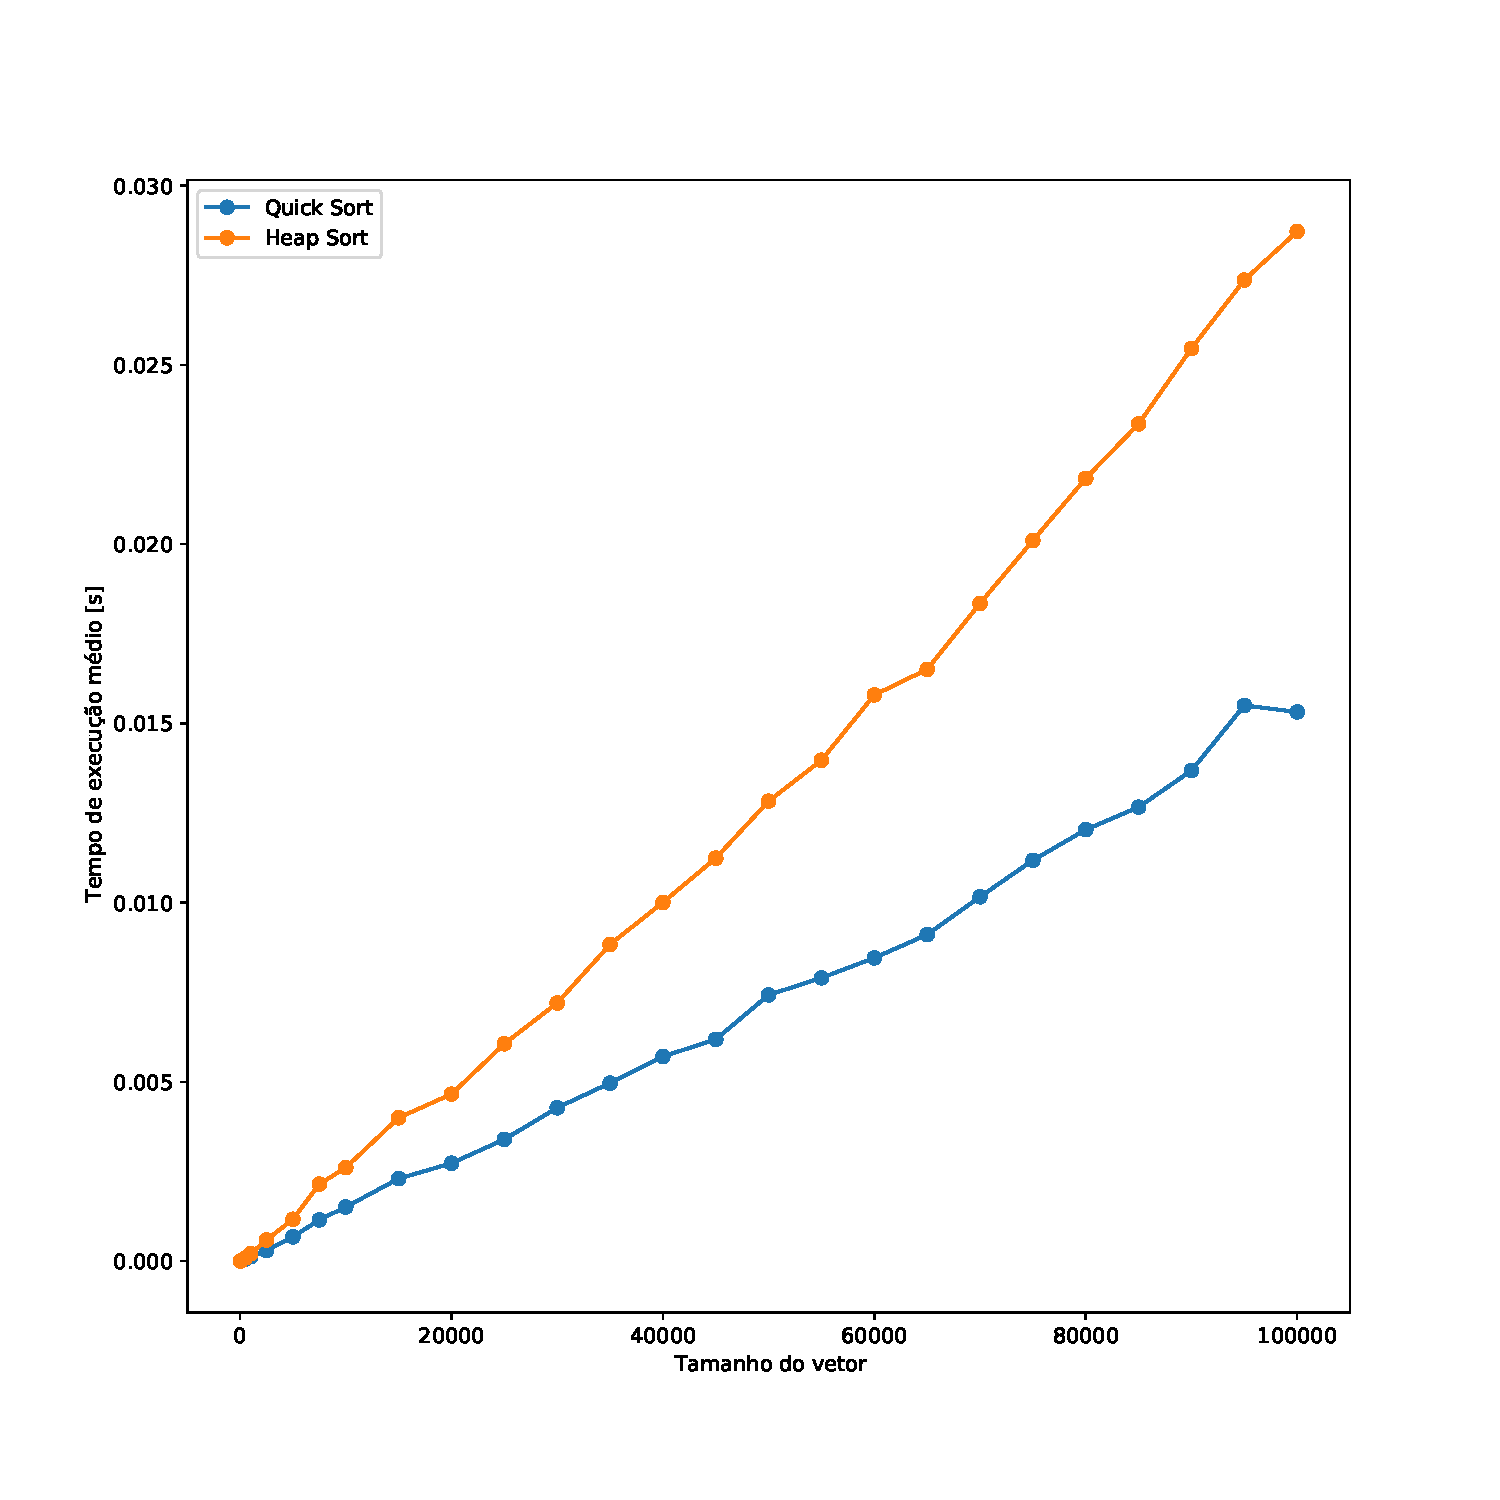
\includegraphics[scale=0.5]{comparacao_1.pdf}
    \caption{Resultado das medições temporais para cada algoritmo; a média de tempo de execução foi tirada a partir de 10 iterações para cada tamanho de vetor.}
    \label{Figura 1}
\end{center}
\end{figure}

\quad Ao observar o gráfico acima, podemos notar que, como esperado, ambos os algoritmos tem comportamento parecido, com caso médio de complexidade de tempo $n \cdot logn$. O $quicksort$, no entanto, mostrou-se significativamente mais rápido em todos os casos.

%%%%% 3.2 COMPARAÇÃO %%%%%
\newpage
\subsection{Comparação com Bubble Sort, Insertion Sort e Merge Sort}

\quad O segundo experimento foi realizado seguindo os mesmos critérios de geração aleatória do teste anterior. Desta vez, no entanto, foram testados simultaneamente os cinco algoritmos (Blubble, Insertion, Merge, Quick e Heap Sort) e a ordenação só foi executada para vetores de tamanho até $n = 50000$, devido à lentidão do \textit{bubblesort} na ordenação de vetores tão grandes. Os resultados do teste são apresentados abaixo.

\begin{table}[!htbp]
\centering
\begin{tabular}{@{}r|ccccc@{}}
\multicolumn{1}{c|}{Tamanho}    & \multicolumn{5}{c}{Tempo de execução médio {[}s{]}}                                                             \\
\multicolumn{1}{c|}{da entrada} & \textbf{Bubble Sort} & \textbf{Insertion Sort} & \textbf{Merge Sort} & \textbf{Quick Sort} & \textbf{Heap Sort} \\ \midrule
25                              & 0.000002             & 0.000002                & 0.000003            & 0.000002            & 0.000002           \\
100                             & 0.000029             & 0.000010                & 0.000011            & 0.000007            & 0.000011           \\
500                             & 0.000591             & 0.000208                & 0.000099            & 0.000043            & 0.000093           \\
1000                            & 0.002292             & 0.000790                & 0.000152            & 0.000095            & 0.000159           \\
2500                            & 0.013896             & 0.004848                & 0.000398            & 0.000264            & 0.000438           \\
5000                            & 0.067162             & 0.019546                & 0.000970            & 0.000600            & 0.000991           \\
7500                            & 0.162504             & 0.044578                & 0.001386            & 0.000943            & 0.001560           \\
10000                           & 0.288760             & 0.077497                & 0.001842            & 0.001212            & 0.002088           \\
15000                           & 0.684054             & 0.174053                & 0.002813            & 0.001871            & 0.003275           \\
20000                           & 1.273150             & 0.318072                & 0.003952            & 0.002687            & 0.004660           \\
25000                           & 1.972511             & 0.479805                & 0.004920            & 0.003353            & 0.006163           \\
30000                           & 2.846070             & 0.699651                & 0.006232            & 0.004282            & 0.007359           \\
35000                           & 3.981880             & 0.948351                & 0.007336            & 0.004790            & 0.008591           \\
40000                           & 5.245678             & 1.242266                & 0.008018            & 0.005444            & 0.009695           \\
45000                           & 6.629168             & 1.607736                & 0.009417            & 0.006244            & 0.011173           \\
50000                           & 8.188427             & 1.966531                & 0.010312            & 0.007138            & 0.012641          
\end{tabular}
\caption{Resultado das medições temporais para cada algoritmo; a média de tempo de execução foi tirada a partir de 10 iterações para cada tamanho de vetor, com vetores gerados aleatoriamente.}
\label{Tabela 2}
\end{table}

\quad Podemos observar que, como esperado pelo que foi demonstrado no item 2 deste relatório, o \textit{bubblesort} apresenta o pior desempenho dentre os cinco algoritmos, seguido pelo \textit{insertion sort}, que apresenta um bom desempenho apenas para vetores de tamanho reduzido ($n \leq 100)$. No gráfico a seguir (Figura 2), podemos observar que o \textit{mergesort}, o \textit{quicksort} e o \textit{heapsort} apresentam comportamente bastante similar quando comparados aos outros.

\begin{figure}[H]
\begin{center}
    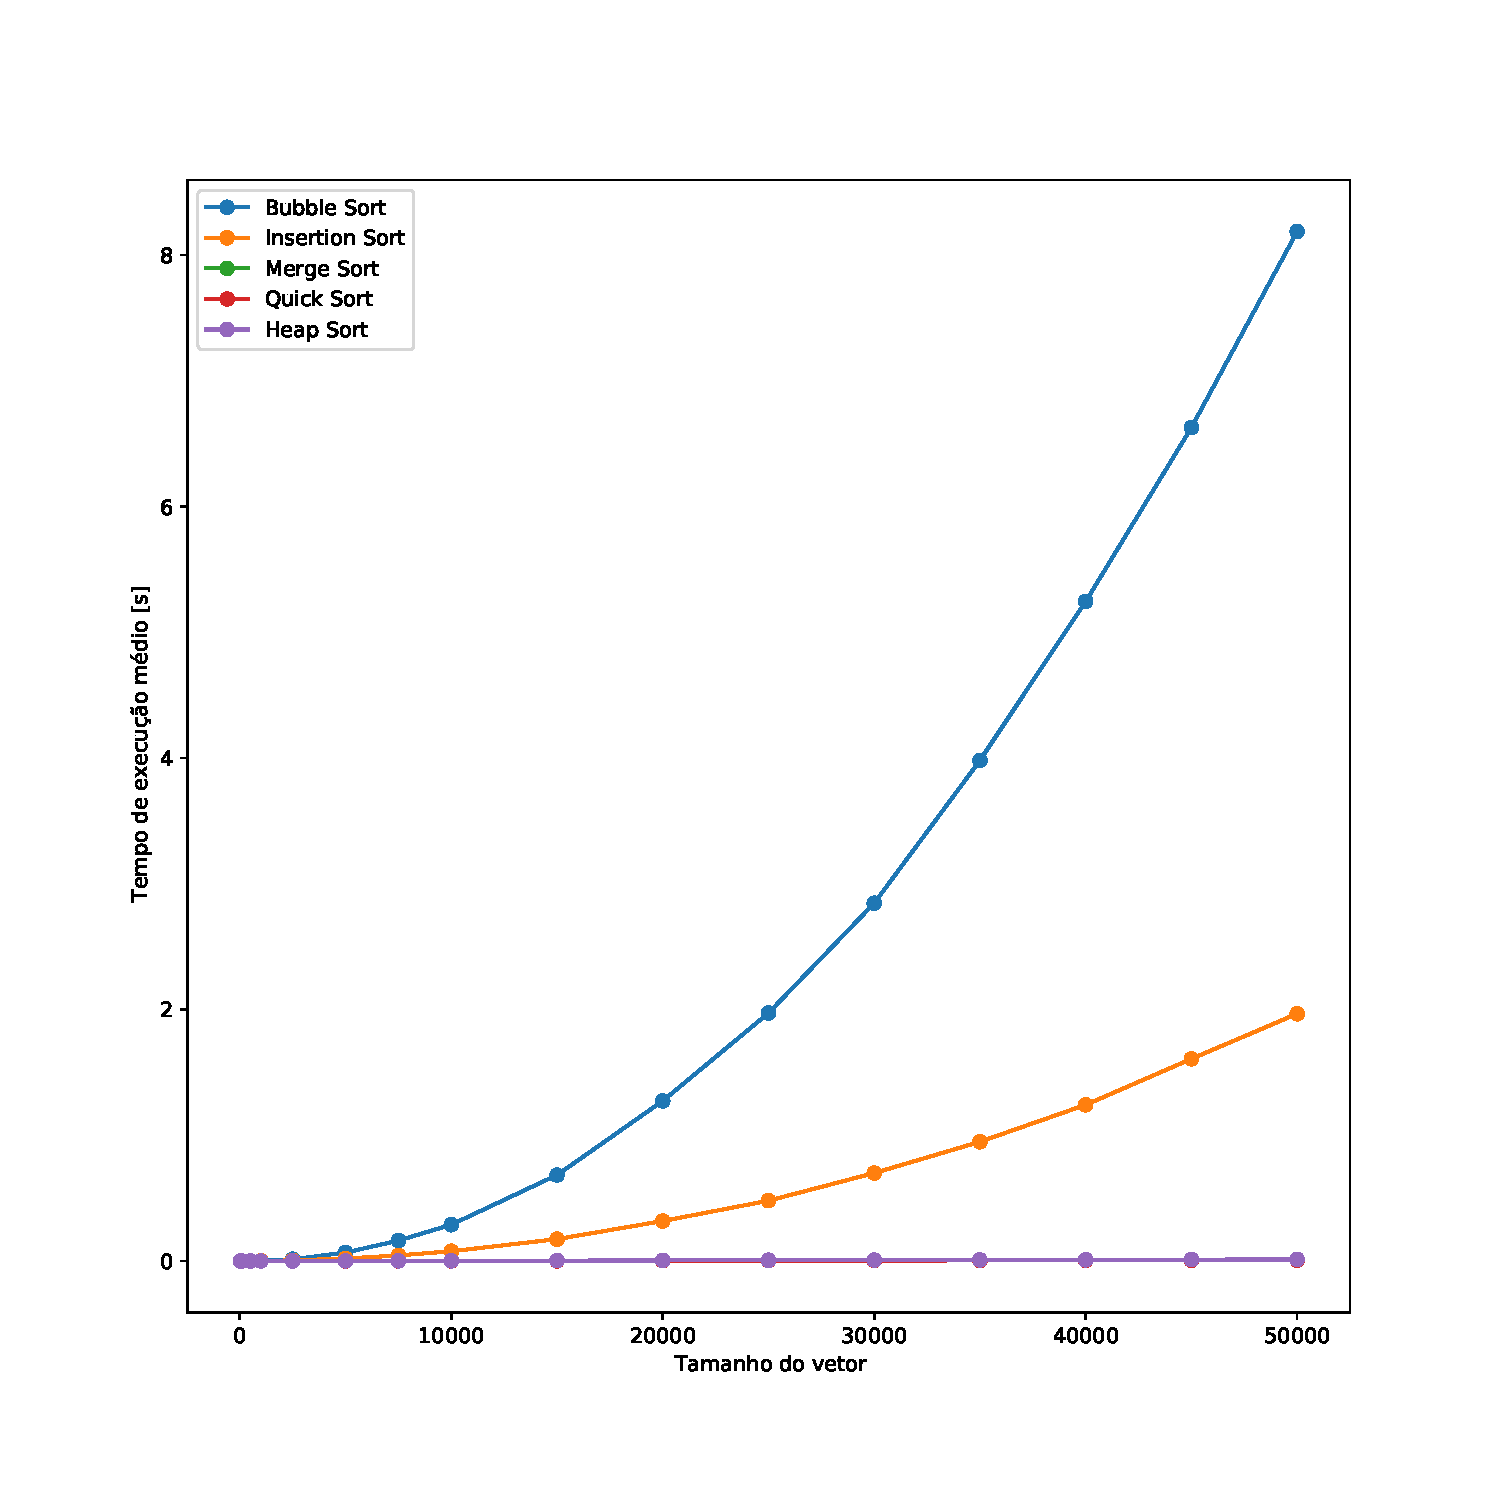
\includegraphics[scale=0.5]{comparacao_2.pdf}
    \caption{Resultado das medições temporais para cada algoritmo; a média de tempo de execução foi tirada a partir de 10 iterações para cada tamanho de vetor.}
    \label{Figura 2}
\end{center}
\end{figure}

\quad Para melhor observar as diferenças entre Merge, Quick e Heap Sort, o gráfico a seguir (Figura 3) compara apenas esses três algoritmos, utilizando os mesmos dados apresentados na Tabela 3 e no gráfico da Figura 2. Podemos notar que, dentre os três, o \textit{quicksort} apresenta o menor tempo médio de execução, seguido pelo \textit{mergesort}; o \textit{heapsort} apresenta o pior desempenho dentre os três.

\begin{figure}[ht]
\begin{center}
    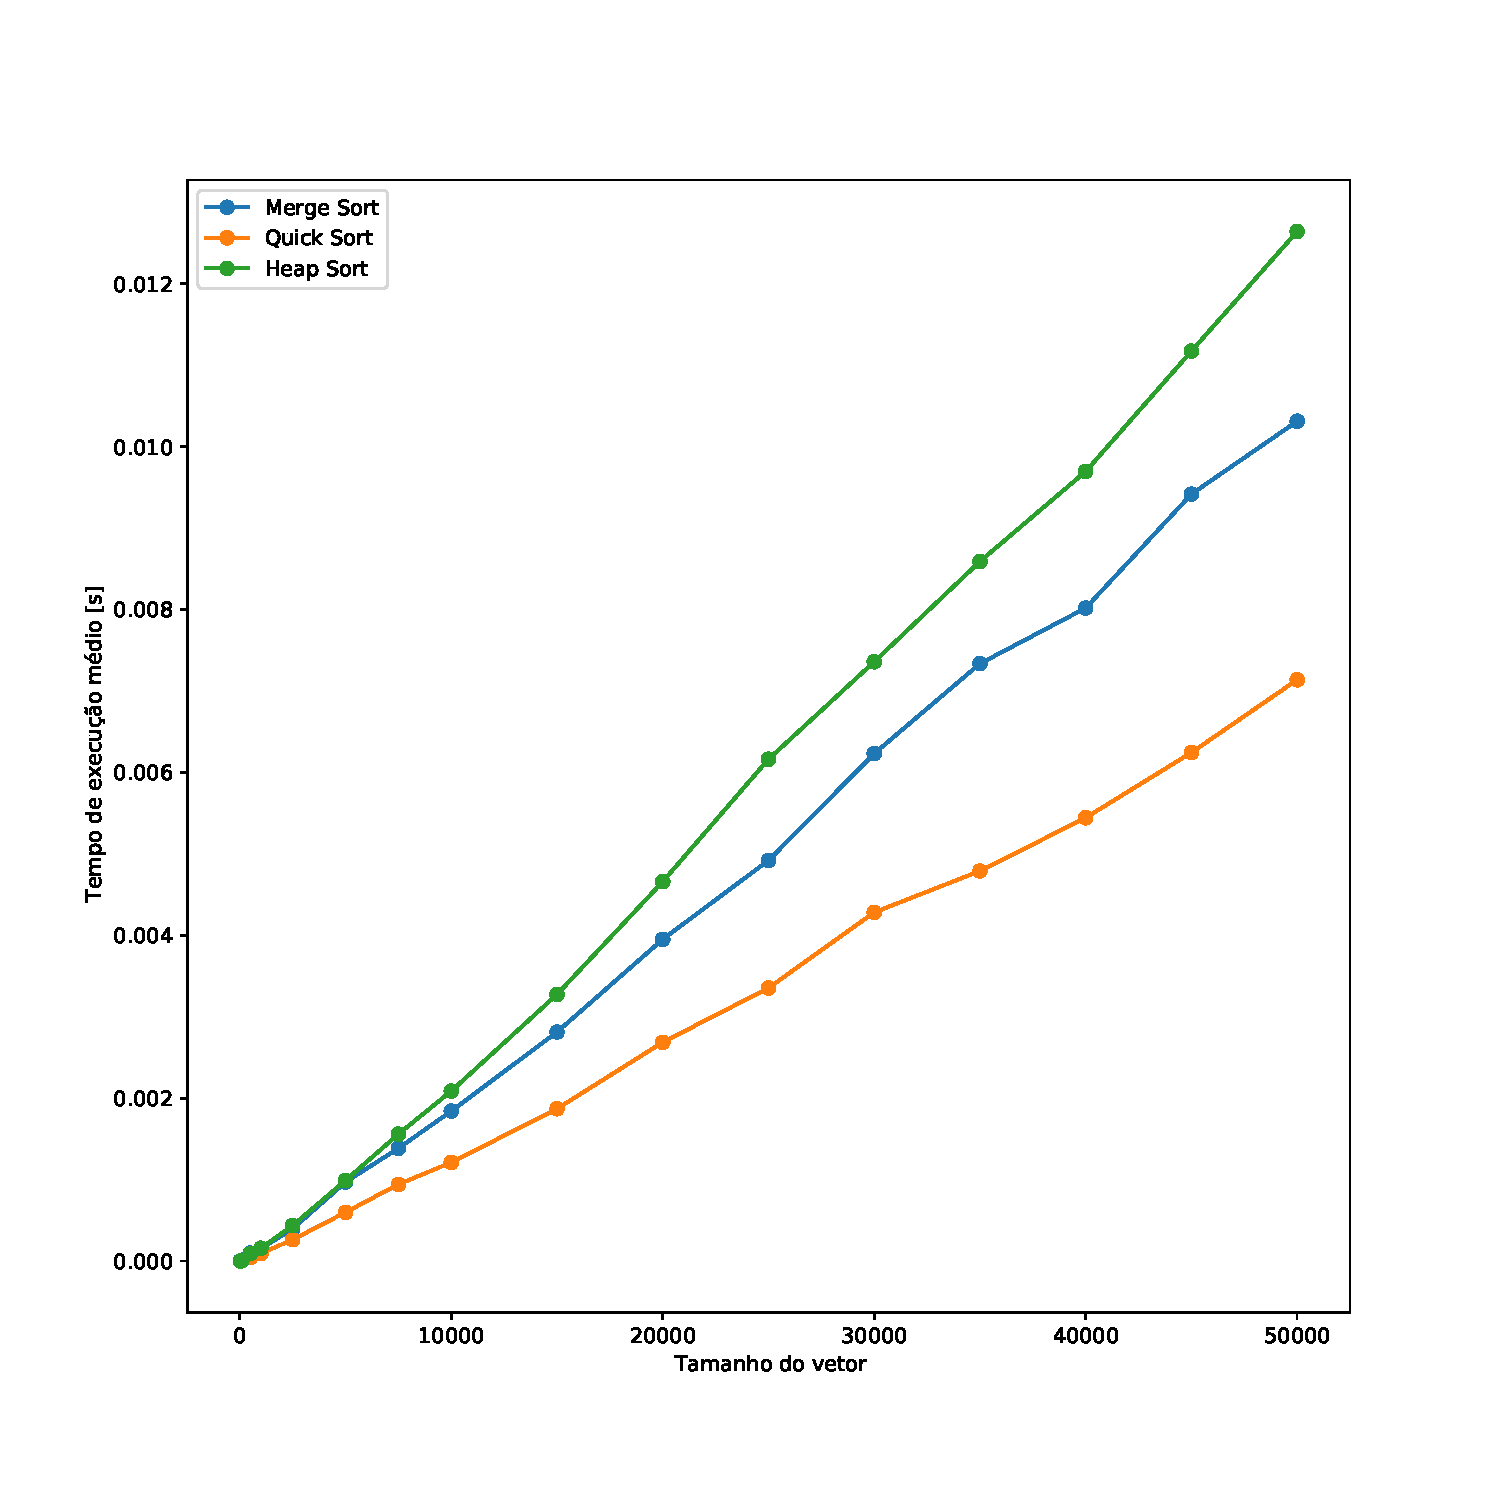
\includegraphics[scale=0.5]{comparacao2_2.pdf}
    \caption{Resultado das medições temporais para cada algoritmo; a média de tempo de execução foi tirada a partir de 10 iterações para cada tamanho de vetor.}
    \label{Figura 3}
\end{center}
\end{figure}

%%%%% 3.3 MELHOR E PIOR CASO %%%%%
\newpage
\subsection{Melhor e pior caso}

\quad Em um terceiro experimento\footnote{Diferentemente do anterior, este teste foi realizado no GDB Online para evitar as otimizações de branch prediction do meu computador (que melhoram o significativamente o desempenho da ordenação no pior caso).}, realizamos testes com vetores de mesmo tamanho ($n = 1000$), porém de diferentes tipos: gerados aleatoriamente, ordenados e inversamente ordenados. De forma complementar aos experimentos anteriores, este teste visou confirmar o que já foi apontado a respeito dos melhores e piores casos para cada algoritmo.

\begin{table}[ht]
\centering
\begin{tabular}{@{}c|ccccc@{}}
Tipo de vetor         & \multicolumn{5}{c}{Tempo de execução médio {[}s{]}}                                                             \\
(tamanho $n = 100$)   & \textbf{Bubble Sort} & \textbf{Insertion Sort} & \textbf{Merge Sort} & \textbf{Quick Sort} & \textbf{Heap Sort} \\ \midrule
Gerado aleatoriamente & 0.002829             & 0.001202                & 0.000184            & 0.000119            & 0.000188           \\
Ordenado              & 0.001492             & 0.000006                & 0.000114            & 0.001255            & 0.000170           \\
Inversamente ordenado & 0.003550             & 0.002418                & 0.000114            & 0.001395            & 0.000163          
\end{tabular}
\caption{Resultado das medições temporais para ordenação de diferentes tipos de vetor, todos com o mesmo tamanho; a média de tempo de execução foi tirada a partir de 10 iterações para cada tipo de vetor.}
\label{Tabela 3}
\end{table}

\quad Pelos dados apresentados na tabela acima, podemos confirmar que, de fato, o caso do vetor inversamente ordenado é o pior caso tanto para o \textit{bubblesort} quanto para o \textit{insertion sort}. Por outro lado, o vetor ordenado é o melhor caso também para ambos, ainda que, como esperado, a diferença entre o melhor e o pior caso seja muito mais expressiva no \textit{insertion sort}. No caso do \textit{mergesort}, podemos observar que não há diferença considerável entre os tempos de execução para diferentes tipos de vetor\footnote{Apesar de o caso do vetor gerado aleatoriamente ter apresentado maior tempo médio de execução, considero que os dados estejam ainda consistentes com o esperado, pois a diferença entre as médias nos três casos é muito pequena.}.

\quad O \textit{quicksort}, como esperado, apresenta o pior desempenho quando testado com vetores ordenados (sejam eles ordenados de maneira crescente ou decrescente). Já o \textit{heapsort}, da mesma maneira que o \textit{merge}, apresenta desempenho similar na ordenação dos três tipos de vetores, não possuindo melhor ou pior caso.

%%%%%%%%%%%%%%%%%%%%%%%%%%%%%%%%%%%%%%%%%%%%%%%%%%%%%%%%%%%
%%%                     4 CONCLUSÃO                     %%%
%%%%%%%%%%%%%%%%%%%%%%%%%%%%%%%%%%%%%%%%%%%%%%%%%%%%%%%%%%%
\section{Conclusão}
    %%%%%% Conclusão do relatório. O que você aprendeu nessa tarefa? %%%%%%
    
\quad Através dos resultados dos experimentos, pudemos confirmar as análises apresentadas no Item 2 deste relatório. Retomando rapidamente o que já foi levantado a respeito do Bubble e do Insertion Sort:

\begin{itemize}
    \item O \textit{bubblesort} é o menos eficiente dos algoritmos em termos de tempo de execução e número de operações executadas; quanto à memória utilizada, apresenta vantagem em relação ao \textit{mergesort} por não utilizar memória auxiliar. No entanto, seu desempenho é muito inferior aos outros e a sua utilização não é recomendada.
    
    \item Em termos de tempo de execução e número de operações executadas, o \textit{insertion sort} mostrou-se melhor que o \textit{bubblesort} e pior que os outros três; quanto ao uso de memória, apresenta vantagem em relação ao \textit{mergesort} por não necessitar de memória auxiliar, da mesma forma que os outros quatro algoritmos. Também observa-se que este é um algoritmo bastante eficiente para entradas suficientemente pequenas ($n \leq 100$).
\end{itemize}

\quad Os outros três algoritmos (\textit{mergesort}, \textit{quicksort} e \textit{heapsort}) possuem ótimo desempenho em termos de tempo de execução e a escolha entre os três deve observar diferenças mais sutis. Em suma:

\begin{itemize}
    \item O tempo de execução médio do \textit{quicksort} é o menor dentre os três e ele não necessita de memória auxiliar em seu funcionamento. No entanto, possui a desvantagem de apresentar casos patológicos, quando os vetores de entrada já estão ordenados ou majoritariamente ordenados, podendo atingir a complexidade de $\mathcal{O}(n^2)$. Esse problema pode ser mitigado por otimizações na escolha do pivô.
    
    \item Dentre os três, aquele que apresenta o segundo melhor tempo de execução é o \textit{mergesort}. Em relação ao \textit{quicksort}, apresenta a vantagem de não encontrar casos patológicos, mas também a desvantagem de necessitar de memória auxiliar para executar a ordenação. Dessa forma, não é recomendada a sua utilização quando há escassez de memória.
    
    \item O \textit{heapsort} apresenta o terceiro melhor desempenho dentre os algoritmos estudados. Apesar de ser mais lento que o \textit{quicksort} e o \textit{mergesort}, configura-se como uma opção segura quando se quer evitar tanto os piores casos do \textit{quicksort} quando a utilização de memória auxiliar demandada pelo \textit{mergesort}.
\end{itemize}


%%%%%%%%%%%%%%%%%%%%%%%%%%%%%%%%%%%%%%%%%%%%%%%%%%%%%%%%%%%
%%%                     REFERÊNCIAS                     %%%
%%%%%%%%%%%%%%%%%%%%%%%%%%%%%%%%%%%%%%%%%%%%%%%%%%%%%%%%%%%
\newpage
\nocite{*}
\bibliographystyle{unsrt}
\bibliography{references.bib}
    %%%%%% Lembre-se de adicionar as referências bibliográficas utilizadas no arquivo 'references.bib'e depois cita-las nessa seção. Conulta: https://pt.overleaf.com/learn/latex/Bibliography_management_in_LaTeX %%%%%%

\end{document}